\documentclass{scrartcl}

\usepackage{amssymb}
\usepackage{amsmath}
\usepackage{tikz}
\usepackage{pgfplots}

%Zou, J. \& L\"{u}, J. (2014). ``The Research of County Urbanization and County Economy Development: Based on 44 Agricultural Counties in Liaoning Province.'' 2014 Fourth International Conference on Instrumentation and Measurement, Computer, Communication and Control, pp. 388-92

\begin{document}
	
	%\begin{figure}
	%	\centering
	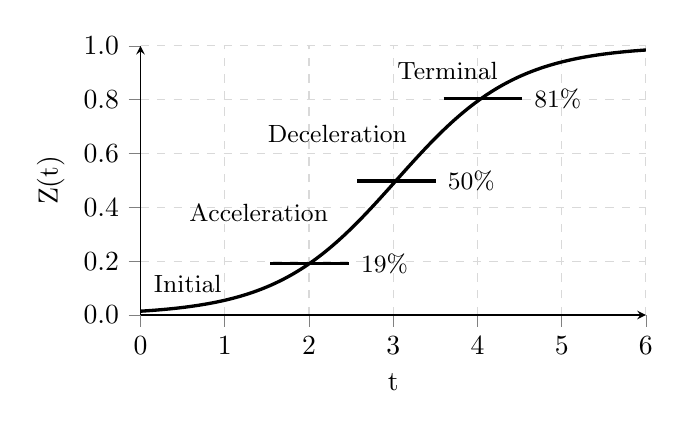
\begin{tikzpicture}
	\begin{axis}[
	axis x line=bottom,
	axis y line=left,
	x tick label style={/pgf/number format/fixed,
		/pgf/number format/fixed zerofill,
		/pgf/number format/precision=0},
	y tick label style={/pgf/number format/fixed,
		/pgf/number format/fixed zerofill,
		/pgf/number format/precision=1},
	grid = major,
	width=8cm,
	height=5cm,
	grid style={dashed, gray!30},
	xmin= 0,	%start diagram at this x-coordinate
	xmax= 6,	%end diagram at this x-coordinate
	ymin= 0,	%start diagram at this y-coordinate
	ymax= 1,	%end diagram at this y-coordinate
	%axis background/.style={fill=white},
	xlabel=t,
	ylabel=Z(t),
	tick align=outside,
	enlargelimits=false]
	% plot the logistic formula (NB: tweaked it to span vertical axis)
	\addplot[domain=0:6,very thick,samples=500] {1/(1+exp(-((1.4*x)-4.25)))};
%	\addplot[domain=0:6,very thick,samples=500] {1/(1+exp(-(x-3)))};	%x-3 b/c 3 is center
	\end{axis}
	\draw[very thick] (3.85,2.75)--(4.85,2.75);	\node at (5.3,2.75) {\small 81\%};
	\draw[very thick] (2.75,1.70)--(3.75,1.70);	\node at (4.2,1.70) {\small 50\%};
	\draw[very thick] (1.65,0.65)--(2.65,0.65);	\node at (3.1,0.65) {\small 19\%};
	\node at (0.6,0.4) {\small Initial};
	\node at (1.5,1.3) {\small Acceleration};
	\node at (2.5,2.3) {\small Deceleration};
	\node at (3.9,3.1) {\small Terminal};
	\end{tikzpicture}
%	\caption{Urbanization as logistic curve (Zou \& L\"{u}, 2014: 390)}
%	\label{fig:sigmoid}
%	\end{figure}
	
\end{document}